\def\tutdate{10.01.2018}

\documentclass[handout]{beamer}
\usepackage{../templates/beamerthemekitwide}
%\usepackage{enumitem}

\usepackage[utf8]{inputenc}
\usepackage[T1]{fontenc}
\usepackage[ngerman]{babel}
\usepackage{listings}
\usepackage{hyperref}
\usepackage{graphicx}

\usepackage{amsmath}
\usepackage{amsthm}
\usepackage{amssymb}
\usepackage{polynom}

%\usepackage{ifthen}
%\usepackage{adjustbox} % for \adjincludegraphics

%\usepackage{tikz}
\usepackage{listings}

%\usepackage[]{algorithm2e}

%\usepackage{colortbl}
\usepackage{verbatim}
%\usepackage{alltt}
%\usepackage{changes}

%\usepackage{pdfpages}
%\usepackage{tabularx}

%\usepackage{euler}


\newcommand{\markBlue}[1]{\textcolor{kit-blue100}{#1}}
\newcommand{\markGreen}[1]{\textcolor{kit-green100}{#1}}
\newcommand{\vertspace}{\vspace{.2cm}}

%\newcommand{\#}{\markBlue{#1}}

%\newcommand{\pitem}{\pause\item}
\newcommand{\p}{\pause}

% -- MATH MACROS
\newcommand{\thistheoremname}{}
\newcommand{\G}{\mathbb{Z}}
\newcommand{\B}{\mathbb{B}}
\newcommand{\R}{\mathbb{R}}
\newcommand{\N}{\mathbb{N}}
\newcommand{\Q}{\mathbb{Q}}
\newcommand{\C}{\mathbb{C}}
\newcommand{\Z}{\mathbb{Z}}
\newcommand{\F}{\mathbb{F}}
\newcommand{\mi}{\mathrm{i}}
\renewcommand{\epsilon}{\varepsilon}
\newcommand{\okalk}{\mathscr{O}}


\newenvironment<>{taskblock}[1]{%
	\setbeamercolor{block title}{fg=kit-orange15,bg=kit-orange100}
	\setbeamercolor{block body}{fg=black,bg=kit-orange30}%
	\begin{block}#2{#1}}{\end{block}}

\setbeamertemplate{enumerate items}[default]

% Aussagenlogik Symbole
\newcommand{\W}{w}
\renewcommand{\F}{f}

% Kodierung
\newcommand{\frepr}{\textbf{repr}}
\newcommand{\fRepr}{\textbf{Repr}}
\newcommand{\fZkpl}{\textbf{Zkpl}}
\newcommand{\fbin}{\textbf{bin}}
\newcommand{\fdiv}{\textbf{ div }}
\newcommand{\fmod}{\textbf{ mod }}

% Speicherabbild
\newenvironment{memory}{\begin{tabular}{r | l}Adresse&Wert\\\hline\hline}{\end{tabular}}
\newcommand{\memrow}[2]{#1 & #2 \\\hline}

% Praedikatenlogik
\newcommand{\objequiv}{\stackrel{\cdot}{=}}
\newcommand{\pval}{val_{D,I,\beta}}

% Neue Befehle
\newcommand{\ip}{\pause} % inline pause, für mitten im satz
\newcommand{\pitem}{\pause\item} % für aufzählungen
\newcommand{\bp}{\pause} % block pause, für zwischen blöcken
\title[Grundbegriffe der Informatik]{ICPC\\Gruppe 2}
\date{\tutdate}
\subtitle{\tutTitle}
\author{Elias Schaut, Dennis Kobert, Niklas Kniep, Lam Vo, Ilia Bozhinov}

\institute{}

\titleimage{bg}
%\titleimage{bg-advent}

%
\ifthenelse{\equal{\compiletype}{livebeamer}}
	{
		\def\livebeamermode{1}
	}{}

\ifthenelse{\equal{\compiletype}{print}}
	{
		\def\printmode{1}
	}{}

\setbeamercovered{invisible}

%\usepackage[citestyle=authoryear,bibstyle=numeric,hyperref,backend=biber]{biblatex}
%\addbibresource{templates/example.bib}
%\bibhang1em

	
\def\tutTitle{O-Notation}
\begin{document}

\selectlanguage{ngerman}

%title page
\begin{frame}
	\titlepage
\end{frame}

\section{Komplexitätstheorie}

\begin{frame}{Komplexitätstheorie}
	\pause
	Wichtige Komplexitätsmaße:
	\begin{itemize}
		\pitem Speicherplatzbedarf
		\pitem Rechen- bzw. Laufzeit
	\end{itemize}
	Unterscheidung in
	\begin{itemize}
		\pitem Best Case (oft uninteressant)
		\pitem Average Case (schwierig zu finden, deswegen selten angegeben)
		\pitem Worst Case  (meistens angegeben)
	\end{itemize}
\end{frame} 

\subsection{O-Notation}
\begin{frame}{Ignorieren konstanter Faktoren}
	\begin{block}{Definition}
		Seien $g,f: \mathbb{N}_0 \rightarrow \mathbb{R}_0^+$ Funktionen. Dann wächst $g$ asymptotisch genauso schnell wie $f$ genau dann, wenn gilt:\\
		$\exists c, c' \in \mathbb{R}_+ : \exists n_0 \in \mathbb{N}_0: \forall n \geq n_0 : c \cdot f(n) \leq g(n)\leq c' \cdot f(n)$
	\end{block}
	\pause

	\textbf{Notation}\\
	$f \asymp g$ oder $f(n) \asymp g(n)$ ("asymptotisch gleich")\\
	\textbf{Bemerkung}\\
	$\asymp$ ist eine Äquivalenzrelation
\end{frame}

\begin{frame}{Theta}
	\begin{block}{Definition}
		$\Theta (f) = \{g|g \asymp f\}$
	\end{block}

	\pause
	
	\begin{block}{Satz}
		$\forall a, b \in \mathbb{R}_+ : \Theta (a\cdot f) = \Theta (b \cdot f)$
	\end{block}
\end{frame}

\begin{frame}{Obere und untere Schranke}
	\begin{block}{Obere Schranke (Worst-Case Approximation)}
		$O(f) = \{g| \exists c \in \mathbb{R}_+ : \exists n_0 \in \mathbb{N}_0: \forall n \geq n_0 : g(n)\leq c \cdot f(n)\}$
	\end{block}

	\pause
	
	\begin{block}{Untere Schranke (Best-Case Approximation)}
		$\Omega(f) = \{g| \exists c \in \mathbb{R}_+ : \exists n_0 \in \mathbb{N}_0: \forall n \geq n_0 : g(n)\geq c \cdot f(n)\}$
	\end{block}
	\pause
	\textbf{Notation}\\
	\begin{itemize}
		\item $g\curlyeqprec f$ falls $g \in O(f)$ bzw. g wächst asymptotisch höchstens so schnell wie f
		\item $g \curlyeqsucc f $ falls $g \in \Omega (f)$ bzw. g wächst asymptotisch mindestens so schnell wie f
	\end{itemize}
	\pause
	\textbf{Bemerkung}\\
	Es gilt $\Theta (f) = O(f) \cap \Omega (f)$
\end{frame}

\begin{frame}
	\begin{block}{Lemma}
		$log_a n \in \Theta (log_b n)$
	\end{block}
	\textbf{Beispiel}\\
	$log_2 n \in \Theta(log_8 n)$\\
	\pause
	\textbf{Beweis}\\
	$\frac{1}{3} log_2 n \ip= \frac{1}{log_2 8} log_2 n \ip= \frac{log_2 n}{log_2 8} \ip= log_8 n \leq log_2 n$
\end{frame}

\begin{frame}
	\textbf{Aufgabe}\\
	Gilt $log_2(n^{20}) \in \Theta (log \space n)$\\
	\pause
	\textbf{Lösung}\\
	Ja, denn $log_2 (n^{20}) = 20 \cdot log_2 n$
\end{frame}

\begin{frame}{Algorithmus von Warshall}
	\begin{columns}
		\begin{column}{0.7\textwidth}
			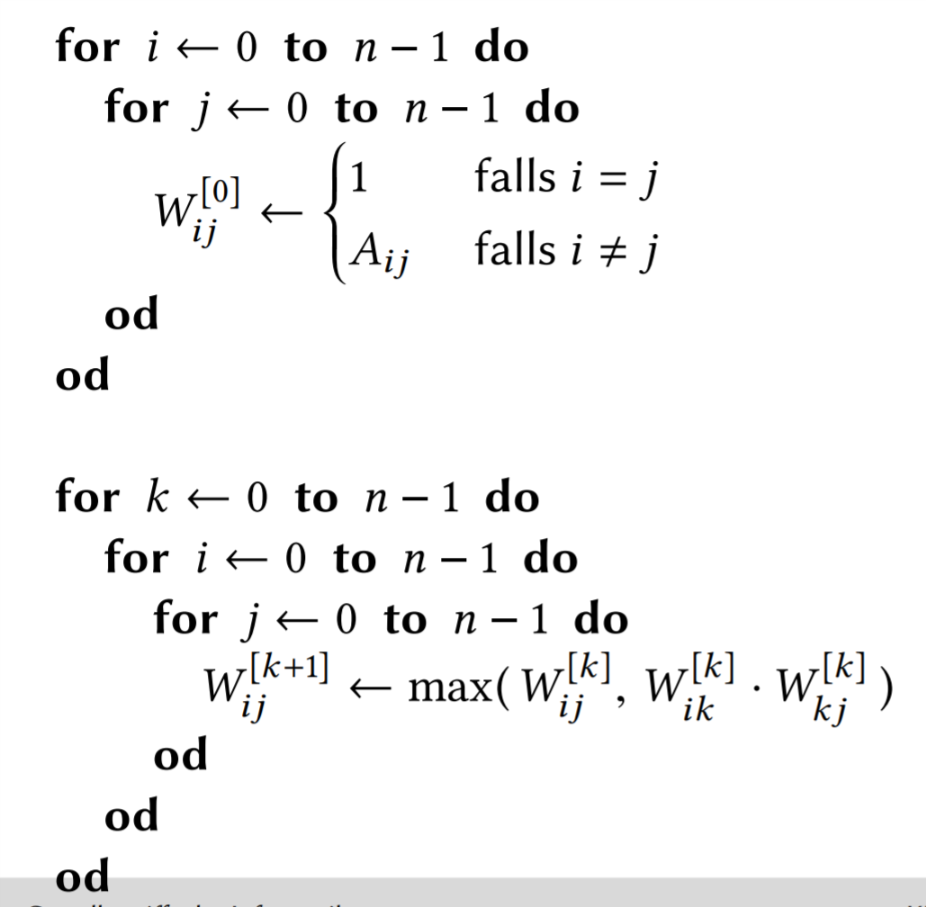
\includegraphics[scale=0.5]{images/warshall.png}\\
		\end{column}
		\begin{column}{0.3\textwidth}
			Wie schnell ist das ganze?
		\end{column}
	\end{columns}
\end{frame}

\begin{frame}
Gelten folgende Approximationen?

\begin{itemize}
	\pitem $4n^2 + \pi n + 2 \sqrt{n} \in \Theta(n^2)?$ \pause Ja.
	\pitem $4n^{2,1} + \pi n + 2 \sqrt{n} \in \Theta(n^2)?$ \pause Nein.
\end{itemize}

\bp Es sind immer nur die höchsten Faktoren interessant!

\begin{itemize}
	\pitem $4n^4 + 3c^6 \in \Theta(n^4)$? \pause Ja\ip, $c$ ist eine Konstante, $3c^6=(3c^6)n^0$ hat eine kleinere Potenz als $n^4$.
	\pitem $\log_{4213}(n) \in \Theta(\log_2(n))$ \pause Ja\ip, die Basis des Logarithmus ist im O-Kalkül egal.
	
	\begin{itemize}
		\pitem Grund: $\okalk(\log_b n) \ip= \okalk(\frac{\log_a n}{\log_a b}) \ip = \okalk(\frac{1}{\log_a b}\log_a n) \ip = \okalk(\log_a n)$.
	\end{itemize}
	
	\pitem $n! \in \Theta(n^{\pi e 2000})$ \pause Nein\ip, Fakultät wächst asymptotisch schneller als fast alles andere.
\end{itemize}
\end{frame}

\begin{frame}{Aufgabe}
\begin{taskblock}{Übungsaufgabe}
Entscheide für jede Zelle, ob die Formel der Zeile in der Menge der Spalte liegt.

\begin{center}
\begin{tabular}{r||c|c|c|c|c|c}%*{2}{>{$}c<{$}}|*{4}{>{$}c<{$}}
	\hline
	& $\okalk(n^3)$ & $\okalk(n)$ & $\Theta(c!)$ & $\Theta(n^\pi)$ & $\Omega(n^6)$ & $\Omega(n!)$ \\\hline\hline
	
	$2n^2 + 4n$ 
	& \visible<2->{$\in$}
	& \visible<3->{$\not\in$}
	& \visible<4->{$\not\in$}
	& \visible<5->{$\not\in$}
	& \visible<6->{$\not\in$}
	& \visible<7->{$\not\in$}
	\\\hline
	
	
	$\pi$
	& \visible<8->{$\in$}
	& \visible<9->{$\in$}
	& \visible<10->{$\in$}
	& \visible<11->{$\not\in$}
	& \visible<12->{$\not\in$}
	& \visible<13->{$\not\in$}
	\\\hline
	
	$\log(n)$
	& \visible<14->{$\in$}
	& \visible<15->{$\in$}
	& \visible<16->{$\not\in$}
	& \visible<17->{$\not\in$}
	& \visible<18->{$\not\in$}
	& \visible<19->{$\not\in$}
	\\\hline
	
	$n\log(n)$
	& \visible<20->{$\in$}
	& \visible<21->{$\not\in$}
	& \visible<22->{$\not\in$}
	& \visible<23->{$\not\in$}
	& \visible<24->{$\not\in$}
	& \visible<25->{$\not\in$}
	\\\hline
	
	$n^\pi$
	& \visible<26->{$\not\in$}
	& \visible<27->{$\not\in$}
	& \visible<28->{$\not\in$}
	& \visible<29->{$\in$}
	& \visible<30->{$\not\in$}
	& \visible<31->{$\not\in$}
	\\\hline
	
	$12n^3+7000n^2$
	& \visible<32->{$\in$}
	& \visible<33->{$\not\in$}
	& \visible<34->{$\not\in$}
	& \visible<35->{$\not\in$}
	& \visible<36->{$\not\in$}
	& \visible<37->{$\not\in$}
	\\\hline
	
	$n^3$
	& \visible<38->{$\in$}
	& \visible<39->{$\not\in$}
	& \visible<40->{$\not\in$}
	& \visible<41->{$\not\in$}
	& \visible<42->{$\not\in$}
	& \visible<43->{$\not\in$}
	\\\hline
	
	$n!$
	& \visible<44->{$\not\in$}
	& \visible<45->{$\not\in$}
	& \visible<46->{$\not\in$}
	& \visible<47->{$\not\in$}
	& \visible<48->{$\in$}
	& \visible<49->{$\in$}
	\\\hline
	
	%\visible<1->{\F} & \visible<1->{\F} & \visible<5->{\F} & \visible<9->{\F} & \visible<17->{\W} & \visible<13->{\F} \\\hline
	
\end{tabular}
\end{center}
\end{taskblock}
\end{frame}


\begin{frame}{Schnitt}
\begin{itemize}
\pitem $\okalk (n^2) \cap \okalk(n) = \okalk(?)$? \pause $= \okalk(n)$.
\pitem $\okalk(n^2) \cap \Omega(n^3) = \pause \emptyset$
\end{itemize}
\end{frame}

\begin{frame}{Grundlegende Reihenfolge von Größen}
\begin{center}
$1 \curlyeqprec \log n \curlyeqprec n \curlyeqprec n \log n \curlyeqprec n^2 \curlyeqprec n^3 \curlyeqprec n^{10000} \curlyeqprec 2^n \curlyeqprec 3^n \curlyeqprec 1000^n \curlyeqprec n! \curlyeqprec n^n$
\end{center}
\end{frame}

\begin{frame}{Mathematische Definitionen}
\begin{align*}
f(n) \in \Omega(g(n)) \Leftrightarrow 0 < \liminf_{n \rightarrow \infty} \frac{f(n)}{g(n)} \leq \infty\\
f(n) \in \Theta(g(n)) \Leftarrow  0 <  \lim_{n \rightarrow \infty} \frac{f(n)}{g(n)} = c < \infty\\
f(n) \in \mathcal{O}(g(n)) \Leftrightarrow 0 \leq \limsup_{n \rightarrow \infty} \frac{f(n)}{g(n)} = c < \infty
\end{align*}

\bp

\begin{taskblock}{Zeige}
% Aufgaben sind vom ersten Algo Blatt letzten Jahres, Lösung: https://crypto.iti.kit.edu/fileadmin/User/Lectures/Algorithmen_SS16/loesung_01.pdf
\begin{itemize}
\item $3n^2 + 14n + 159 \in \Theta(n^2)$ %a1 a i
\item $\log n^2 \in \Theta(\log n^3)$ %a1 b ii
\item $\log^2 n \in \okalk(\log^3 n)$ %a1 b i
\end{itemize}
\end{taskblock}
\end{frame}

%\begin{frame}{Komplexität mit vollständiger Induktion beweisen}
% Ebenfalls vom Algo blatt. Vielleicht nur kurz zeigen bzw vorrechnen, eher nur um nochmal vollst Induktion zu zeigen.

%\begin{taskblock}{Zeige mittels vollständiger Induktion}
%\begin{itemize}
%\item $2^n \in \Omega(n^3)$ %a1 a ii
%\item $(n+1)! \in \okalk(n! + 2^n)$ %a1 b iii
%\end{itemize}
%\end{taskblock}
%\end{frame}

\begin{frame}
\begin{tabular}{| r || l |}
\hline Größenordnung & Bezeichnung\\\hline\hline\ip 

$\okalk(1)$ & konstante Laufzeit \\\hline\ip 
$\okalk(\log n)$ & logarithmische Laufzeit \\\hline\ip 
$\okalk(\log^2 n)$ & quadratisch logarithmische Laufzeit \\\hline\ip 
$\okalk(n)$ & lineare Laufzeit \\\hline\ip 
$\okalk(n^2)$ & quadratische Laufzeit \\\hline\ip 
$\okalk(n^3)$ & kubische Laufzeit \\\hline\ip 
$\okalk(n^k)$ & polynomielle Laufzeit \\\hline
\end{tabular}
\end{frame}


\begin{frame}
	
\includegraphics[width=\linewidth]{../images/thatsall.png}
\end{frame}


\end{document}